\documentclass{bioinfo}
\copyrightyear{2015} \pubyear{2015}

\access{Advance Access Publication Date: Day Month Year}
\appnotes{Manuscript Category}

\begin{document}
\firstpage{1}

\subtitle{Subject Section}

\title[PMMP]{A graph-based approach for modification site assignment in proteomics}
\author[Sample \textit{et~al}.]{Dafni Skiadopoulou\,$^{\text{\sfb 1,2}}$, Lukas Käll\,$^{\text{\sfb 3}}$, and Marc Vaudel\,$^{\text{\sfb 1,2,4,}*}$}
\address{$^{\text{\sf 1}}$Mohn Center for Diabetes Precision Medicine, Department of Clinical Sciences, University of Bergen, Bergen, Norway, and \\
$^{\text{\sf 2}}$Computational Biology Unit, Department of Informatics, University of Bergen, Bergen, Norway, \\
$^{\text{\sf 3}}$Science for Life Laboratory, School of Engineering Sciences in Chemistry, Biotechnology and Health, KTH Royal Institute of Technology, Stockholm, Sweden, and \\
$^{\text{\sf 4}}$Department of Genetics and Bioinformatics, Health Data and Digitalization,
Norwegian Institute of Public Health, Oslo, Norway.}

\corresp{$^\ast$To whom correspondence should be addressed.}

\history{Received on XXXXX; revised on XXXXX; accepted on XXXXX}

\editor{Associate Editor: XXXXXXX}

\abstract{\textbf{Summary:} 
	Assigning protein post-translational modifications to acceptor sites requires the distribution of modifications in a way that maximizes localization scores while avoiding chemically impossible configurations. We provide an efficient graph-based approach to this problem implemented both as standalone implementation and integrated in the PeptideShaker interface. \\
\textbf{Availability and Implementation:} 
	An open source implementation in Python is available at https://github.com/ProGenNo/peptides-modifications-matching under a GPL-3.0 license. An open source implementation in Java is available at github.com/compomics/compomics-utilities under an Apache-2.0 license. \\
\textbf{Contact:} \href{dafni.skiadopoulou@uib.no}{marc.vaudel@uib.no}\\
\textbf{Supplementary information:} Supplementary data are available at \textit{Bioinformatics}
online.}

\maketitle

\section{Introduction}

Tandem mass spectrometry (MS/MS) has become the reference tool for the identification of proteins from a sequence database. For that, the observed spectra of peptide fragments are matched against theoretical spectra to determine the proteins that are expressed in a biological mixture. This process becomes much more difficult when it comes to modified proteins because even a small change in the amino acids sequence can lead to a significant shift in the peaks of the corresponding spectrum. Such changes can be the product of post-translational modifications (PTMs) or mutations of the proteins which also result in alterations of the protein's functionality. Except of finding the types of the existing PTMs in a protein, another crucial aspect of the identification process is to determine the exact sites in the amino acid chain where the modifications are located. 

This problem of modification site localization has been addressed by several tools starting from the Ascore \citep{AScore} that was mainly used for phosphorylation localization, which uses only site-determining fragment ions present in an MS/MS spectrum to create a probability-based score that a site is correctly localized. {\bf ...... continue with past related work overview .......}


Tandem mass spectrometry (MS/MS) has become the reference approach for the identification of proteins from a sequence database. Proteins can be modified, which alters their function, and can be detected by mass shifts at specific sites of the amino acid sequence. While the identification of modified proteins can be achieved by considering the modification of every possible acceptor site, the exponential increase of the search space makes the accurate assignment of modifications to sites intractable for highly modified proteins like histones. 
Here, a graph modeling approach is presented that considers the possibilities of modifications occurring at specific sites of the amino acid chains, and returns the most likely modification sites with controlled processing time. The modification assignment problem is reduced to the Maximum Weight Matching (MWM) problem in bipartite graphs, using modification localization probabilities as weights.

\section{Past-related work}

The Ascore \citep{AScore} metric uses only site-determining fragment ions present in an MS/MS spectrum to create a probability-based score that a site is correctly localized.

ModLS \citep{ModLS} calculates the PTM score (proposed in \citep{PTMScore}) of each localization combination and then for the top-ranked localization the final value is the difference in PTM Score between this and the second ranked.

In the work of \citep{pSite} a semi-supervised SVM model is used to estimate the confidence of each amino acid obtained by de novo peptide sequencing which is also proved to yield accurate results for the modification site localization problem.

A Site Localization In Peptide (SLIP) scoring is proposed by \citep{SLIP} that is automatically calculated for all modifications in peptides identified by the search engine Batch-Tag in the Protein Prospector suite of tools.

Using mass accuracy and peak intensities, LuciPHOr tool \citep{LuciPHOr} improves site localization and false localization rate (FLR) estimation. It estimates FLR based on a target-decoy framework, in which artificial phosphorylation is used to generate decoy phosphopeptides to compare with target matches from a database search.

In the work of \citep{MSFragger} the search engine MSFragger is extended with a shifted ion indexing strategy that enables localization-aware open search leading to an increased number of identified PSMs and an improvement in accuracy at the detection of single amino acid substitutions.

PTM-Shepherd \citep{PTM-Shepherd} manages to determine which PSMs contain a specific mass shift and characterizes PTM profiles in open searches using attributes such as amino acid localization, fragmentation spectra similarity and retention time.

The PTMiner \citep{PTMiner} tool can be used to assist in localizing the potential mass modifications discovered during open modification searches (....have to describe how this is done....).




%\citep{Bag01} wants to know about
%{\ldots}{\ldots} text follows.
%\begin{equation}
%\sum \text{\it x}+ \text{\it y} =\text{\it Z}\label{eq:01}\vspace*{-10pt}
%\end{equation}

%\enlargethispage{12pt}

\section{Approach}

In this work the modification site localization problem is addressed by a graph theoretical approach. For each studied peptide a weighted bipartite graph ($G = \{V,E,w\}$) is used to model all possible combinations of modifications on the amino acid chain. In this graph we determine two kinds of vertices, the ones that represent the different modifications that have occured in the peptide (ie $D = \{d_1, d_2, \dots, d_k\}$) and the ones that represent all their possible acceptor sites in the amino acid chain (ie $A = \{a_1, a_2, \dots, a_n\}$). The set of the graph's vertices $V$ is then formed by the union of the sets $A$ and $D$ (ie $V = A \cup D$). For each modification, an edge is formed between the corresponding vertex and the ones that represent its possible acceptor sites. Moreover, a weight is assigned to each edge, taking the value of the confidence score (\textbf{is this really a confidence score???}, have to better describe the scores we're using...) which represents the probability of the modification to have occurred in that specific site of the amino acid chain. An example of a graph model for a modified peptide is presented in Fig. \ref{fig:PMMP_model}

Using this graph modeling we can reduce the modification site localization problem to the maximum weight matching problem on the resulting graph. This consists of finding a set of edges that are pairwise non-adjacent (without common vertices), in which the sum of weights is maximized. Solving this problem in the graph model of our application will result in the best combination of modifications localization on the peptide, based on their confidence scores. 

\begin{figure}[!tpb]%figure2
\centerline{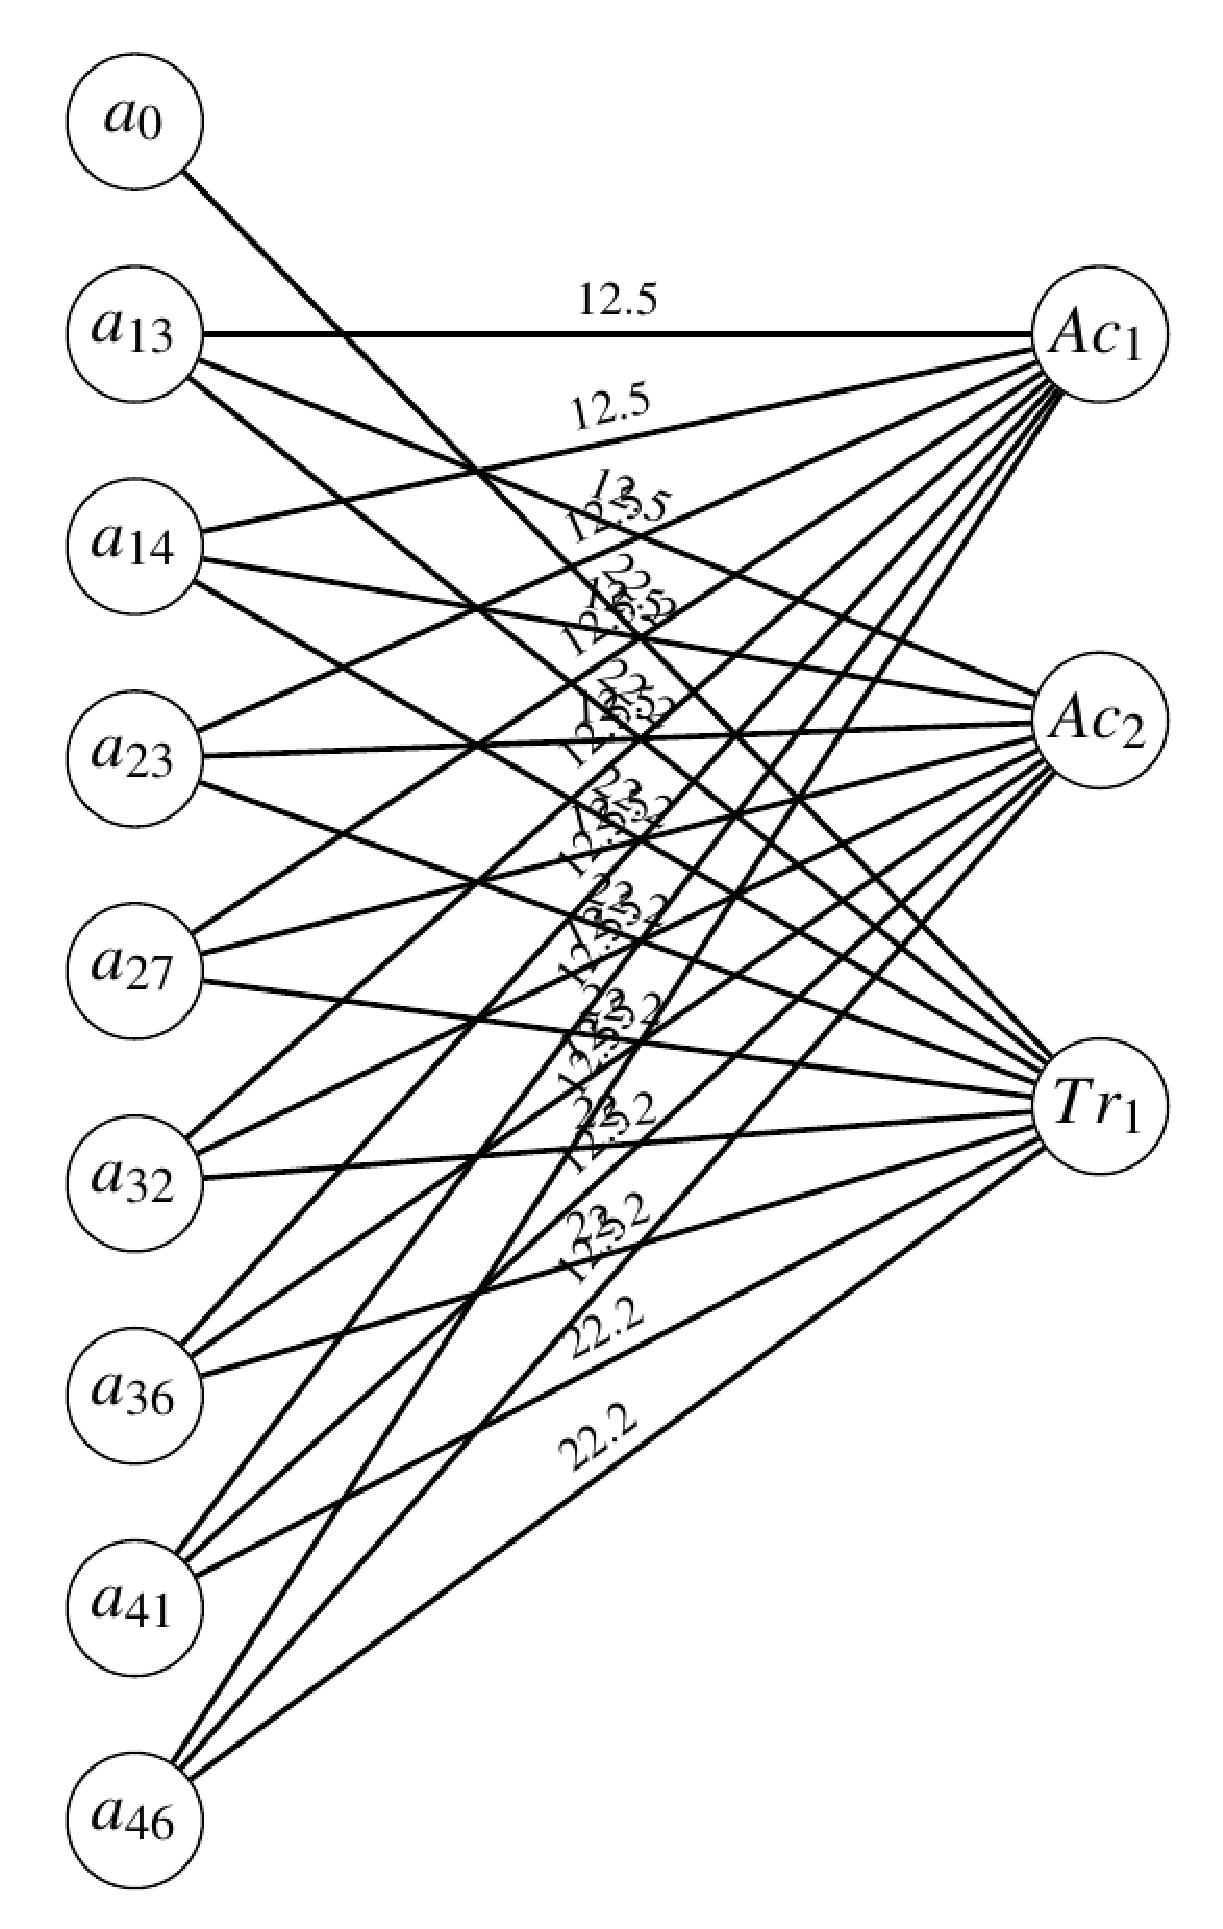
\includegraphics[width=0.2\textwidth]{pmmp_model.eps}}
\caption{Graph representation of a peptide with 2 Acetylations and 1 Trimethylation with all their possible acceptor sites.}\label{fig:PMMP_model}
%RLAVTGPRYRHPKKVGGTSPASKRTAKTALQKRPAKGGTSKRATQKTLA
\end{figure}

%Equation~(\ref{eq:01}) Text Text Text Text Text Text  Text Text
%Figure~2\vphantom{\ref{fig:02}} shows that the above method  Text
%\citealp{Boffelli03} might want to know about text text text text
%.....


\begin{methods}
\section{Methods}

(mention the usage of python's networkX library implementation of the maximum weight matching algorithm based on methods invented by Jack Edmonds 1965 \textbf{???})

%text\vspace*{1pt}

%\begin{itemize}
%\item for bulleted list, use itemize
%\item for bulleted list, use itemize
%\item for bulleted list, use itemize\vspace*{1pt}
%\end{itemize}

%Text Text  Text Text Text Text Text Text\vadjust{\newpage}.

%\subsection{This is subheading}

%\subsubsection{This is subsubheading}


%\enlargethispage{6pt}

%\begin{table}[!t]
%\processtable{This is table caption\label{Tab:01}} {\begin{tabular}{@{}llll@{}}\toprule head1 &
%head2 & head3 & head4\\\midrule
%row1 & row1 & row1 & row1\\
%row2 & row2 & row2 & row2\\
%row3 & row3 & row3 & row3\\
%row4 & row4 & row4 & row4\\\botrule
%\end{tabular}}{This is a footnote}
%\end{table}

\end{methods}

%\begin{figure}[!tpb]%figure1
%\fboxsep=0pt\colorbox{gray}{\begin{minipage}[t]{235pt} \vbox to 100pt{\vfill\hbox to
%235pt{\hfill\fontsize{24pt}{24pt}\selectfont FPO\hfill}\vfill}
%\end{minipage}}
%\centerline{\includegraphics{fig01.eps}}
%\caption{Caption, caption.}\label{fig:01}
%\end{figure}

%\begin{figure}[!tpb]%figure2
%%\centerline{\includegraphics{fig02.eps}}
%\caption{Caption, caption.}\label{fig:02}
%\end{figure}


%\subsection{Test1}

\section{Results}


%%%%%%%%%%%%%%%%%%%%%%%%%%%%%%%%%%%%%%%%%%%%%%%%%%%%%%%%%%%%%%%%%%%%%%%%%%%%%%%%%%%%%
%
%     please remove the " % " symbol from \centerline{\includegraphics{fig01.eps}}
%     as it may ignore the figures.
%
%%%%%%%%%%%%%%%%%%%%%%%%%%%%%%%%%%%%%%%%%%%%%%%%%%%%%%%%%%%%%%%%%%%%%%%%%%%%%%%%%%%%%%






\section{Conclusion}

%\begin{enumerate}
%\item this is item, use enumerate
%\item this is item, use enumerate
%\item this is item, use enumerate
%\end{enumerate}

%Figure~2\vphantom{\ref{fig:02}} shows\vadjust{\pagebreak} that the
%Text Text Text Text Text Text Text\break Text.

%Figure~2\vphantom{\ref{fig:02}} shows that the above method  Text
%Text Text Text\vspace*{-10pt}


%\section*{Acknowledgements}

%Text Text Text Text Text Text  Text Text.  \citealp{Boffelli03} might want to know about  text
%text text text\vspace*{-12pt}

\section*{Funding}

%This work has been supported by the... Text Text  Text Text.\vspace*{-12pt}

%\bibliographystyle{natbib}
%\bibliographystyle{achemnat}
%\bibliographystyle{plainnat}
%\bibliographystyle{abbrv}
%\bibliographystyle{bioinformatics}
%
%\bibliographystyle{plain}
%
%\bibliography{Document}


\begin{thebibliography}{}

\bibitem[Yu {\it et~al}., 2020]{MSFragger}
Yu,F.T. {\it et~al}. (2020) Identification of modified peptides using localization-aware open search. {\it Nat Commun.}, {\bf 11} (1), 4065.

\bibitem[Yang {\it et~al}., 2018]{pSite}
Yang,H. {\it et~al}. (2018) pSite: Amino Acid Confidence Evaluation for Quality Control of De Novo Peptide Sequencing and Modification Site Localization {\it Journal of Proteome Research}, {\bf 17} (1), 119-128.

\bibitem[Baker {\it et~al}., 2011]{SLIP}
Baker,P.R. {\it et~al}. (2011) Modification site localization scoring integrated into a search engine.
{\it Mol. Cell. Proteomics.}, {\bf 10}, (M111. 008078)

\bibitem[Fermin {\it et~al}., 2013]{LuciPHOr}
Fermin,D. {\it et~al}. (2013) LuciPHOr: algorithm for phosphorylation site localization with false localization rate estimation using modified target-decoy approach. {\it Mol Cell Proteomics}, {\bf 12} (11), 3409-19.

\bibitem[Trudgian {\it et~al}., 2012]{ModLS}
Trudgian,D. {\it et~al}. (2012) ModLS: Post-translational modification localization scoring with automatic specificity expansion. {\it J. Proteomics Bioinform.}, {\bf 5}, 283–289.

\bibitem[Beausoleil {\it et~al}., 2006]{AScore}
Beausoleil,S.A. {\it et~al}. (2006) A probability-based approach for high-throughput protein phosphorylation analysis and site localization. {\it Nat. Biotechnol.}, {\bf 24}, 1285–1292.

\bibitem[Olsen {\it et~al}., 2006]{PTMScore}
Olsen,J.V. {\it et~al}. (2006) Global, in vivo, and site-specific phosphorylation dynamics in signaling networks. {\it Cell.}, {\bf 127} (3), 635-48.




\end{thebibliography}
\end{document}
